
\subsection{Filtros IIR}

\begin{frame}
\frametitle{Procedimiento de diseño de filtros IIR}

\footnotesize

\begin{itemize}
\item Diseño a partir de las aproximaciones de filtros analógicos:

\hspace{2.5cm}\alert{$H_a(s)=\frac{N_a(s)}{D_a(s)}  \:\:\: \rightarrow \:\:\:   H(z)=K \frac{N(z)}{D(z)}$}
\visible<2->{
\begin{itemize}
\footnotesize
\item Aprovechan los avances existentes en la definición de los filtros analógicos (y la existencia de tablas/programas que permiten definirlos)
\item Suelen producir soluciones con forma cerrada (la expresión matemática de la función de transferencia)
\item El procedimiento sirve también para simular el comportamiento de los filtros analógicos antes de construirlos.
\item En algunos casos es necesario normalizar H(z) ya que en la conversión no se conserva que la magnitud máxima sea igual a 1.
\end{itemize}}
\visible<3->{
\item De forma asistida por computador, utilizando algoritmos que optimicen la posición de los polos/ceros del filtro. La optimización suele consistir en minimizar el error entre la respuesta en frecuencia deseada y la del filtro diseñado. Se utiliza para diseñar filtros con prestaciones particulares.
}

\end{itemize}
\end{frame}

%%%%%%%%%%%%%%%%%%%%%%%


\begin{frame}
\frametitle{Transformación del espacio de trabajo ($s \leftrightarrow z$)}
\footnotesize

\begin{itemize}

\item \alert{Filtro continuo $H_a(s)$ $\rightarrow$  filtro discreto: $H(z)=H_a(s)|_{s=F(z)}$}

\visible<2->{
\item Existen diferentes tipos de funciones $s=F(z)$:}

\begin{itemize}
\footnotesize



\visible<3->{
\item \alert{Relación a la respuesta al impulso: $z=e^{Ts}$}
\vspace{-0.2cm}
\begin{columns}[c]
\hspace{1cm}\begin{column}{7cm}
\begin{itemize}
\scriptsize
\item Asigna bandas de anchura $2\pi/T$ en el plano s negativo con puntos dentro la circunferencia unidad en el plano z. Este hecho esta relacionado con el fenómeno del aliasing.

\item Es una correspondencia de muchos (continuo) a uno (discreto).

\item Debido al aliasing, solo sirve para diseñar filtros paso baja y paso banda.

\end{itemize}
\end{column}
\hspace{-0.5cm}\begin{column}{3.5cm}
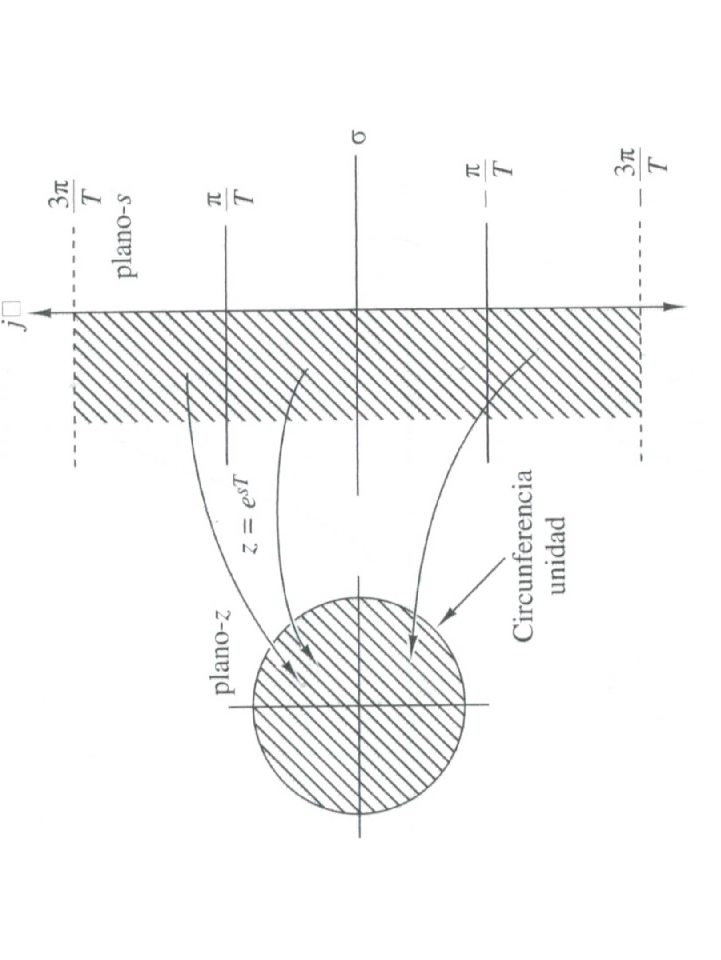
\includegraphics[trim=0cm 1cm 0cm 1cm, clip=true,angle=-90,width=3.5cm]{Figures/Impulso.png}
\end{column}
\end{columns}
}
\visible<4->{
\item \alert{Aproximación por derivadas: $\:\:s= \frac{1-z^{-1}}{T} \: \: \leftrightarrow \:\: z=\frac{1}{1-T\cdot s}$}


\vspace{-0.1cm}
\begin{columns}[c]
\hspace{1cm}\begin{column}{7cm}
\begin{itemize}
\scriptsize
\item Se obtiene sustituyendo la $df(t)/dt$ por $[f(nT)-f((n-1)T)]/T$
\item Puntos del semiplano izquierdo s se relacionan con los puntos internos de la circunferencia pequeña. Se mantiene la estabilidad.
\item Los polos del filtro digital están confinados en la circunferencia pequeña: no se puede diseñar cualquier filtro digital.
\end{itemize}
\end{column}
\hspace{-0.5cm}\begin{column}{3.5cm}
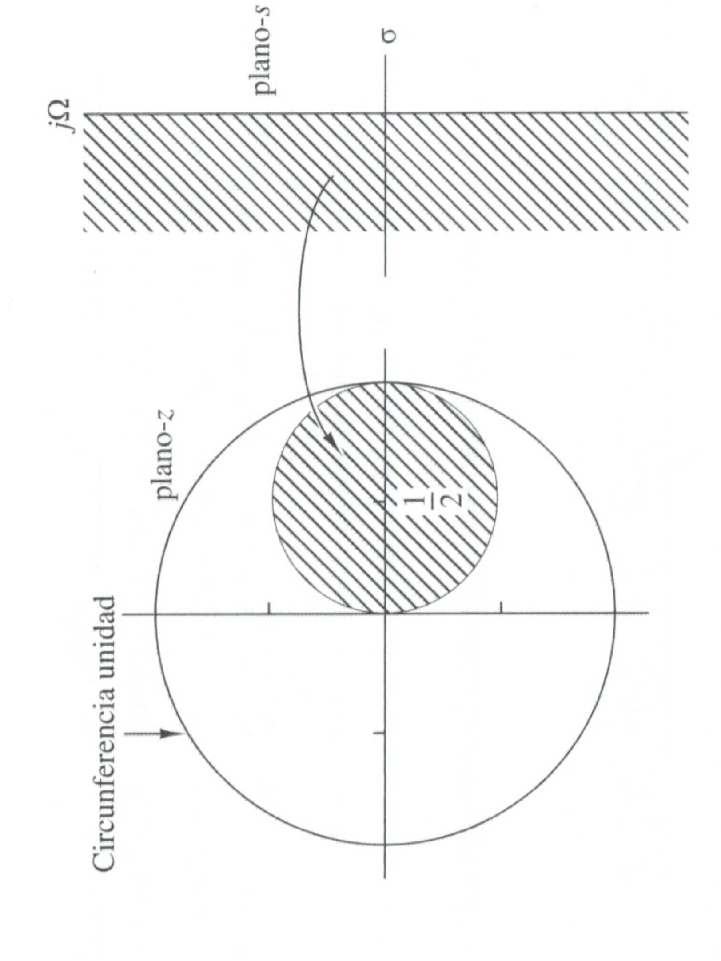
\includegraphics[angle=-90,width=3.5cm]{Figures/Derivada.png}
\end{column}
\end{columns}}
\end{itemize}
\end{itemize}

\end{frame}




%%%%%%%%%%%%%%%%%%%%%%%

\begin{frame}
\frametitle{Transformación del espacio de trabajo ($s \leftrightarrow z$)}
\footnotesize

\begin{itemize}
\item \alert{Filtro continuo $H_a(s)$ $\rightarrow$  filtro discreto: $H(z)=H_a(s)|_{s=F(z)}$}
\item \alert{Transformada bilineal: $\:\:s=\frac{2}{T}\left ( \frac{1-z^{-1}}{1+z^{-1}}\right) \: \: \leftrightarrow \:\: z=\frac{1+T\cdot s/2}{1-T\cdot s/2}$}
\vspace{-0.2cm}
\begin{columns}[T]
\hspace{1cm}\begin{column}{7.5cm}
\begin{itemize}
\scriptsize
\item Se obtiene mediante la aplicación del método de integración numérica trapezoidal a la representación de la ecuación diferencial correspondiente a $H_a(s)$. T es el periodo del paso de integración.

\item Puntos del semiplano izquierdo s se relacionan con los puntos internos a la circunferencia.

\end{itemize}
\end{column}
\begin{column}{4cm}
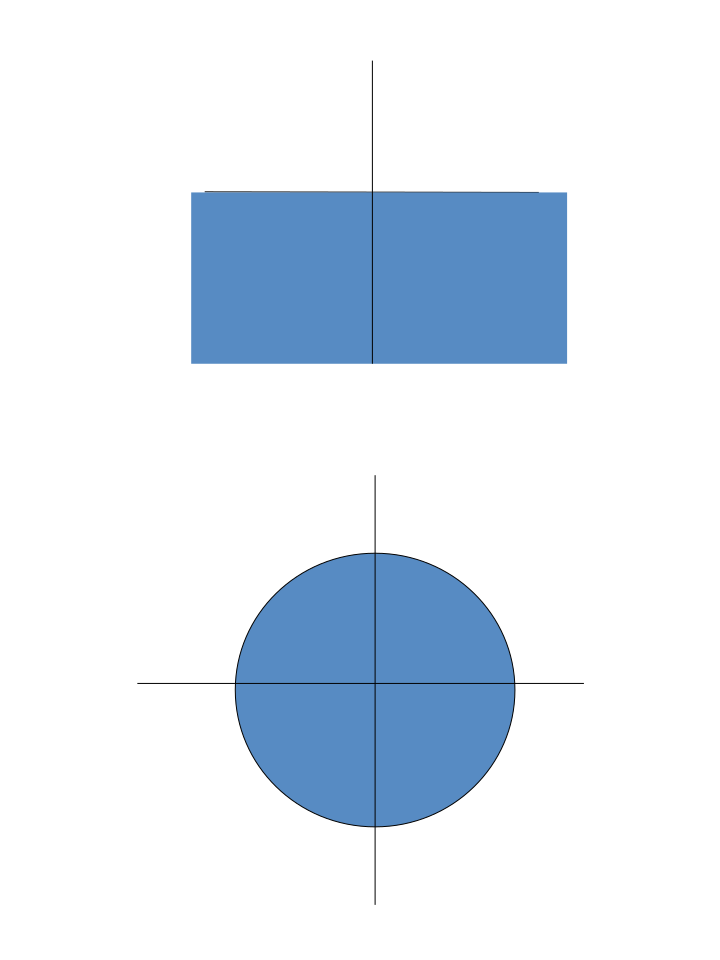
\includegraphics[trim=0cm 0cm 0cm 0cm, clip=true,angle=-90,width=3.5cm]{Figures/Bilineal.png}
\end{column}
\end{columns}


\begin{columns}[T]
\hspace{0.4cm}\begin{column}{11cm}
\begin{itemize}
\scriptsize
\item Es una transformada punto a punto. Se puede utilizar para todos los filtros.

\visible<2->{

\item Relación en frecuencias: \alert{$w_a=\frac{2}{T}tan(w_d/2)$} permite obtener la caracterización del filtro continuo a partir de la caracterización discreta.

\color{gray}
Se establece la relación de s y z con las frecuencias continuas ($s=jw_a$) y discretas ($z=e^{jw_d}$)

$jw_a=\frac{2}{T}\left ( \frac{1-e^{-jw_d}}{1+e^{-jw_d}}\right)=\frac{2}{T}\left ( \frac{e^{jw_d/2}-e^{-jw_d/2}}{e^{jw_d/2}+e^{-jw_d/2}}\right)=\frac{2}{T} j \frac{sen(w_d/2)}{cos(w_d/2)}=\frac{2j}{T} tan(w_d/2)$

Se cumple que  $w_d \!\in \![0,\pi] \leftrightarrow w_a \!\in\! [0,\infty)$; $w_d  \!\in\! [0,-\pi] \leftrightarrow w_a \!\in\! [0,-\infty)$
}
\visible<3->{
\color{black}
\item Se produce un combado de las frecuencias, asociado al comportamiento no lineal de la tangente.
}
\visible<4->{
\item \alert{Si hacemos T=2, las expresiones se simplifican.}
}
\end{itemize}
\end{column}
\end{columns}

\end{itemize}

\end{frame}



%%%%%%%%%%%%%%%%%%%%%%%

\begin{frame}
\frametitle{Diseño de filtros IIR paso bajo}
\small
\begin{enumerate}
\item Aplicar la relación entre las frecuencias ($w_a=\frac{2}{T}tan(w_d/2)$) para obtener la especificación en frecuencias del filtro continuo.
\item Diseñar el filtro continuo correspondiente (Butterworth, Chebyshev, Elíptico). Obtener su función de transferencia $H_a(s)$.
\item Aplicar la transformada bilineal ($s=\frac{2}{T}\left ( \frac{1-z^{-1}}{1+z^{-1}}\right)$) para obtener la función de transferencia del filtro discreto.
\begin{itemize}
\item Con Matlab: \alert{\texttt{[numz,denz]=bilinear(nums,dens,1/T)}}
\end{itemize}

\item Representar la respuesta en frecuencia del filtro (no hay que normalizarlo).
\begin{itemize}
\item Con Matlab: \alert{\texttt{[Hw,w]=freqz(numz,denz)}}


\end{itemize}

\end{enumerate}

\rule{12cm}{0.4pt}
\footnotesize

T=2 para simplificar las expresiones, hacen de la orden bilineal se llamen con tercer parámetro igual a 0.5.

\end{frame}

%%%%%%%%%%%%%%%%%%%%%%%%%%



\begin{frame}
\frametitle{Ejemplo de diseño de filtro  IIR paso bajo}

\footnotesize
\color{olivegreen} Diseñar un IIR de Butterworth paso bajas que opera con una tasa de muestreo de 200 KHz, con una frecuencia de paso de 25KHz y una frecuencia supresora de 55KHz, con un rizo paso banda que no exceda los 0.5 dB y una atenuación mínima en la banda supresora de 15dB.
\color{gray}
\vspace{0.1cm}

1)  Especificaciones del filtro continuo:

\vspace{0.1cm}

$\left . \begin{array}{l}w_{pd}=w_pT_s=2\pi 25/200=0.25\pi\\w_{sd}=w_sT_s=2\pi 55/200=0.55\pi\end{array}\right \}$ $\rightarrow \left . \begin{array}{l}w_{pa}=tan(w_{pd}/2)=0.4142\\w_{sa}=tan(w_{sd}/2)=1.1708\end{array}\right \}$

\vspace{0.1cm}

2) Cálculo del filtro continuo (utilizando expresiones/Matlab):

\vspace{0.1cm}

\hspace{0.3cm}\texttt{[N,wca]=buttord(0.4142,1.1708,.5,15,'s')}

\vspace{0.1cm}

\hspace{0.3cm}\texttt{[numc,denc]=butter(N,wca,'low','s')};

\vspace{0.1cm}

\begin{columns}[T]
\begin{column}{7cm}
3) Conversión al filtro discreto

\vspace{0.1cm}

\hspace{0.3cm}\texttt{[numd,dend]=bilinear(numc,denc,0.5)}

\vspace{0.1cm}

4) Representación del espectro del filtro:

\vspace{0.1cm}

\hspace{0.3cm}\texttt{[Hw,w]=freqz(numz,denz)}

\vspace{0.1cm}

\hspace{0.3cm}\texttt{plot(w/pi,abs(Hw))}
\end{column}
\begin{column}{4cm}

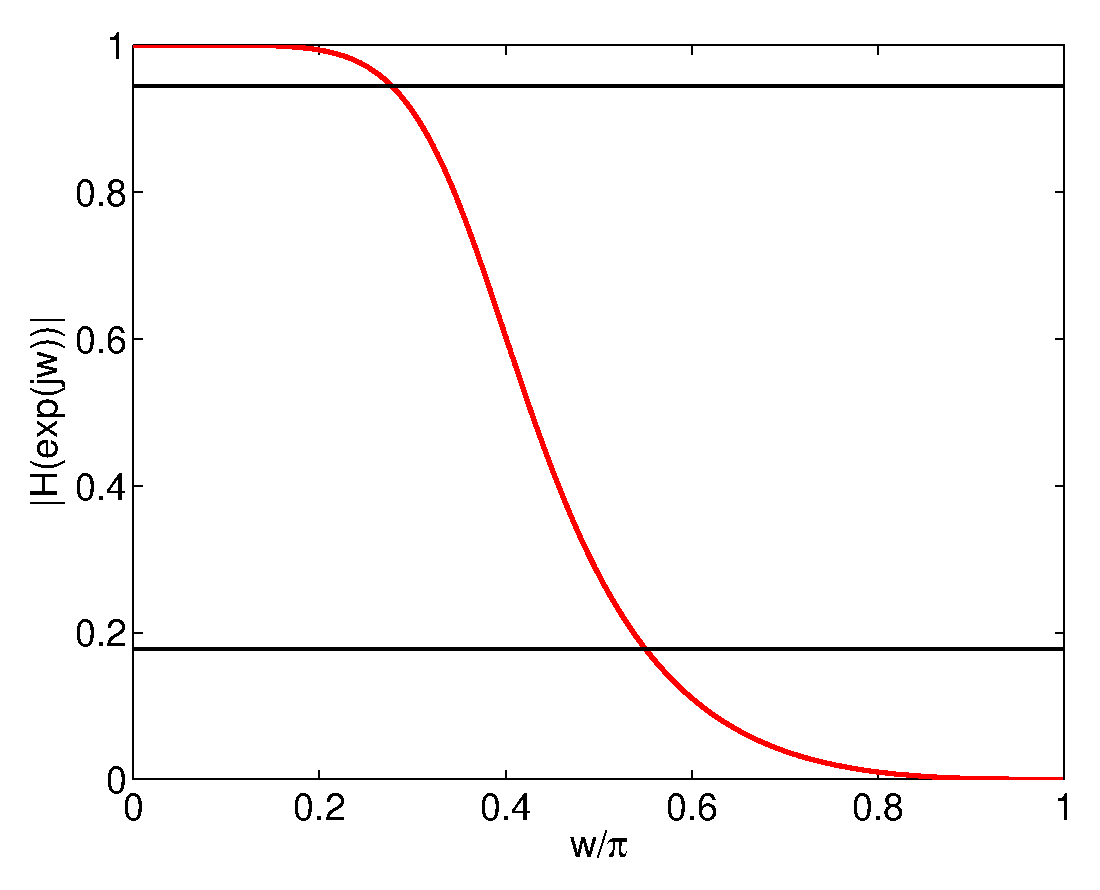
\includegraphics[width=4cm]{Figures/FiltroDiscretoPB_Butter.eps}
\end{column}
\end{columns}


\end{frame}

%%%%%%%%%%%%%%%%%%%%%%%%%%%%


\begin{frame}
\frametitle{Filtros  IIR paso alto, paso banda, supresor de banda}
\small

\visible<2->{
\vspace{-0.4cm}
\begin{enumerate}
\item Aplicar la relación entre las frecuencias ($w_a=\frac{2}{T}tan(w_d/2)$) para obtener la especificación en frecuencias del filtro continuo $H_a(s)$.
\vspace{-0.1cm}
\item Convertir las especificaciones del filtro continuo $H_a(s)$ en las de un filtro paso baja continuo $H_{LP}(s)$.
\vspace{0.1cm}

\begin{columns}[T]
\hspace{0.8cm}\begin{column}{2cm}
\scriptsize
Paso alto:

\vspace{0.2cm}

$s=\frac{w_p \hat w_p}{\hat s}$

\vspace{0.2cm}

 $- w \hat w=w_p \hat w_p$
\end{column}
\hspace{-0.8cm}\begin{column}{3cm}
\scriptsize
Paso banda:

\vspace{0.1cm}

 $s=w_p\frac{\hat s^2+\hat w_0^2}{\hat s (\hat w_{p2}-\hat w_{p1})}$

$w=w_p\frac{\hat w^2-\hat w_0^2}{\hat w (\hat w_{p2}-\hat w_{p1})}$

$\hat w_0^2=\hat w_{p1}\hat w_{p2}=\hat w_{s1}\hat w_{s2}$

\end{column}
\hspace{-0.8cm}\begin{column}{3cm}
\scriptsize
Supresor de banda:

\vspace{0.1cm}

$s=w_s\frac{\hat s (\hat w_{s2}-\hat w_{s1})}{\hat s^2+\hat w_0^2}$

$w=w_s\frac{\hat w (\hat w_{s2}-\hat w_{s1})}{\hat w_0^2-\hat w^2}$

$\hat w_0^2=\hat w_{p1}\hat w_{p2}=\hat w_{s1}\hat w_{s2}$


\end{column}

\end{columns}

\vspace{-0.2cm}

\item Diseñar el filtro continuo paso bajas $H_{LP}(s)$

\vspace{-0.1cm}
}
\visible<4->{
\item Seguir uno de los dos procedimientos siguientes:
}
\end{enumerate}
\vspace{-0.3cm}
\begin{columns}[T]
\begin{column}{5.5cm}
\footnotesize \visible<5->{
\hspace{1.5cm}Procedimiento 1
\begin{itemize}
\scriptsize
\item Convertir el filtro paso baja $H_{LP}(s)$ en el filtro destino $H_a(s)$ usando la relación espectral correspondiente.
\vspace{-0.1cm}
\item  Convertir el filtro $H_a(s)$ en el filtro discreto $H(z)$ con la transformación bilineal ($s=\frac{2}{T}\left ( \frac{1-z^{-1}}{1+z^{-1}}\right)$)
\end{itemize}}
\end{column}
\begin{column}{5.5cm}
\footnotesize \visible<6->{
\hspace{1.5cm}Procedimiento 2
\begin{itemize}
\scriptsize
\item Convertir el filtro paso baja $H_{LP}(s)$ en el filtro $H_{LP}(z)$ con la  transformación bilineal ($s=\frac{2}{T}\left ( \frac{1-z^{-1}}{1+z^{-1}}\right)$).
\vspace{-0.1cm}
\item Convertir el filtro $H_{LP}(z)$ en el filtro destino $H(z)$ usando la relación espectral discreta correspondiente.
\end{itemize}}
\end{column}
\end{columns}
\end{frame}



\begin{frame}
\frametitle{Ejemplo de un filtro  IIR  paso alto}
\footnotesize

\footnotesize
\color{olivegreen} Diseñar con el procedimiento 1 un IIR de Chebyshev Tipo 1 paso altas con las siguientes características: borde de la frecuencia de paso 700Hz, borde de la banda supresora 500Hz, rizo paso banda 1dB, atenuación mínima banda supresora 32 dB, frecuencia de muestreo 2KHz.
\color{gray}
\vspace{0.1cm}

1)  Obtener las especificaciones del filtro continuo paso alta $H_a(s)$:

$\left . \begin{array}{l}w_{pd}=w_pT_s=2\pi 700/2000=0.7\pi\\w_{sd}=w_sT_s=2\pi 500/2000=0.5\pi\end{array}\right \}$ $\rightarrow \left . \begin{array}{l}\hat w_{pa}=tan(w_{pd}/2)=1.9626\\\hat w_{sa}=tan(w_{sd}/2)=1.0\end{array}\right \}$

\vspace{0.1cm}

2) Obtener las especificaciones del filtro continuo paso baja $H_{LP}(s)$:

\vspace{0.1cm}


\hspace{0.25cm}$w\hat w=w_{pa}\hat w_{pa}$. Suponiendo que $w_{pa}=1 \rightarrow w_{sa}=\hat w_{pa}/\hat w_{sa}=1.9626$.

\vspace{0.1cm}

\begin{columns}[T]
 \hspace{0.2cm}\begin{column}{7.7cm}
3) Diseño filtro Chebyshev Tipo 1

\vspace{0.1cm}

\hspace{0.25cm}\texttt{[N,wn]=cheb1ord(1,1.9626,1,32,'s')}

\hspace{0.25cm}\texttt{[numlp,denlp]=cheby1(N,1,wn,'low','s')}

\vspace{0.1cm}

 4) Seguir el procedimiento 1:

 \vspace{0.1cm}

 \hspace{0.25cm}\texttt{[numhp,denhp]=lp2hp(numlp,denlp,1.9626)}

\hspace{0.25cm}\texttt{[numz,denz]=bilinear(numhp,denhp,0.5);}
 \end{column}
 \hspace{-0.5cm}\begin{column}{3.8cm}
 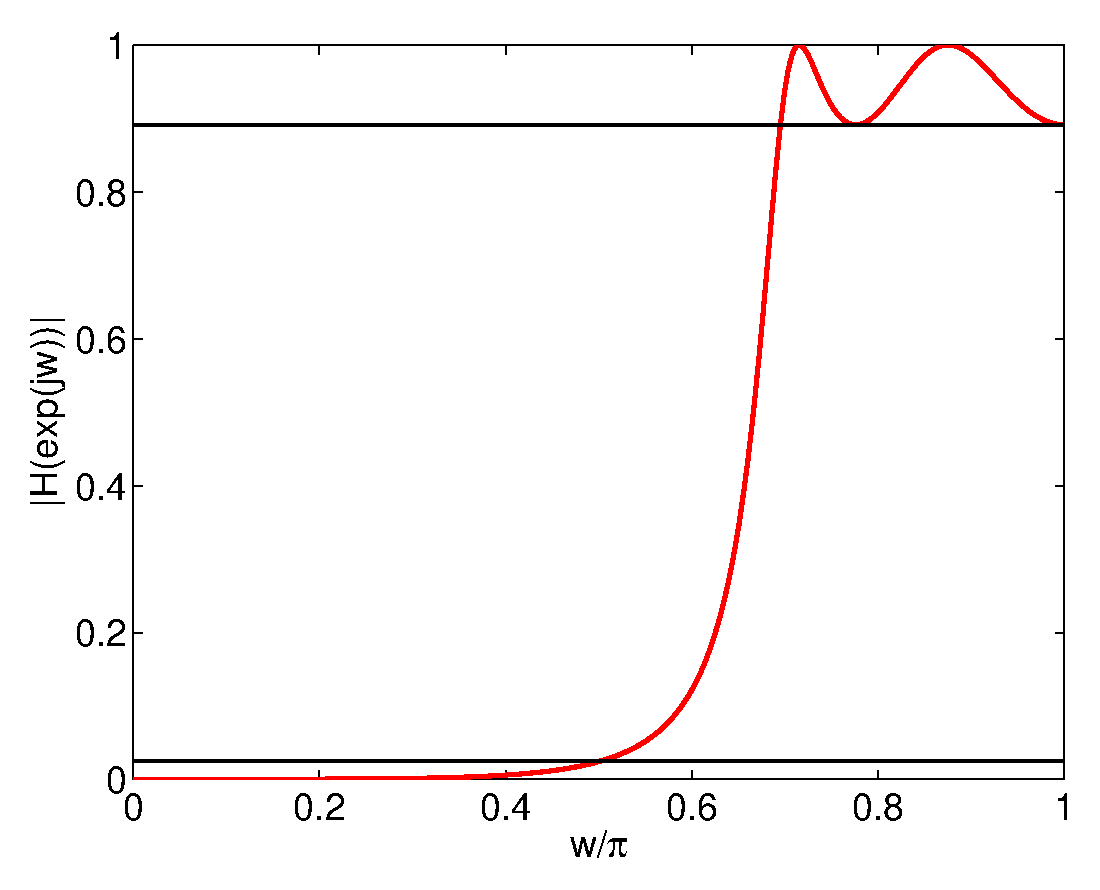
\includegraphics[width=3.8cm]{Figures/FiltroDiscretoPA_Cheby1.eps}
 \end{column}
 \end{columns}

\end{frame}


%%%%%%%%%%%%%%%%%%%%%%%%%%%%%%%%



\begin{frame}
\frametitle{Ejemplo de un filtro  IIR paso banda}
\footnotesize

\footnotesize
\color{olivegreen} Diseñar con el procedimiento 1 un IIR de Butterworth paso banda con las siguientes características: bordes normalizados de la banda de paso 0.45$\pi$ y 0.65$\pi$, bordes normalizados de la banda supresora 0.3$\pi$ y 0.75$\pi$, rizo paso banda 1dB, atenuación mínima banda supresora 40 dB.
\color{gray}
\vspace{0.1cm}

1)  Características del filtro continuo paso banda $H_a(s)$, usando $\hat w_{a}=tan(w_{d}/2)$  :

$\begin{array}{ll}w_{p1d}=0.45\pi \rightarrow \hat w_{p1a}=0.8541 &\:\: w_{p2d}=0.65\pi \rightarrow \hat w_{p2a}=1.6319 \\
w_{s1d}=0.3\pi \rightarrow \hat w_{s1a}=0.5095 &\:\: w_{s2d}=0.75\pi \rightarrow \hat w_{s2a}=2.4142
\end{array}$

\vspace{0.1cm}

2) Obtener las especificaciones del filtro continuo paso baja $H_{LP}(s)$:

\vspace{0.1cm}

$\left . \begin{array}{l}\hat w_0^2 =\hat w_{p1a}\hat w_{p2a}=1.3938\\w_0^2 =\hat w_{s1a}\hat w_{s2a}=1.23
\end{array} \right \}$ $\rightarrow \hat w_{s1a}=\frac{1.3938}{w_{s2a}}=0.5772$, $\hat w_0=1.1806$


\hspace{0.25cm}Si $w_p=1$, $w_{s}=w_p\frac{\hat w_{s1a}^2-\hat w_0^2}{\hat w_{s1a} (\hat w_{p2}-\hat w_{p1})}=2.3617$


\vspace{0.1cm}

\begin{columns}[T]
 \hspace{0.2cm}\begin{column}{7.7cm}
3) Diseño filtro Butterworth

\vspace{0.1cm}

\hspace{0.25cm}\texttt{[N,wn]=buttord(1,2.3617,1,40,'s')}

\hspace{0.25cm}\texttt{[nlp,dlp]=butter(N,wn,'low','s')}

\vspace{0.1cm}

 4) Seguir el procedimiento 1:

 \vspace{0.1cm}
  \hspace{0.28cm}\texttt{banda=1.6139-0.8541;}

 \hspace{0.25cm}\texttt{[npb,dpb]=lp2bp(nlp,dlp,1.1806,banda)}

\hspace{0.25cm}\texttt{[numz,denz]=bilinear(npd,dpd,0.5);}
 \end{column}
 \hspace{-0.5cm}\begin{column}{3.8cm}
 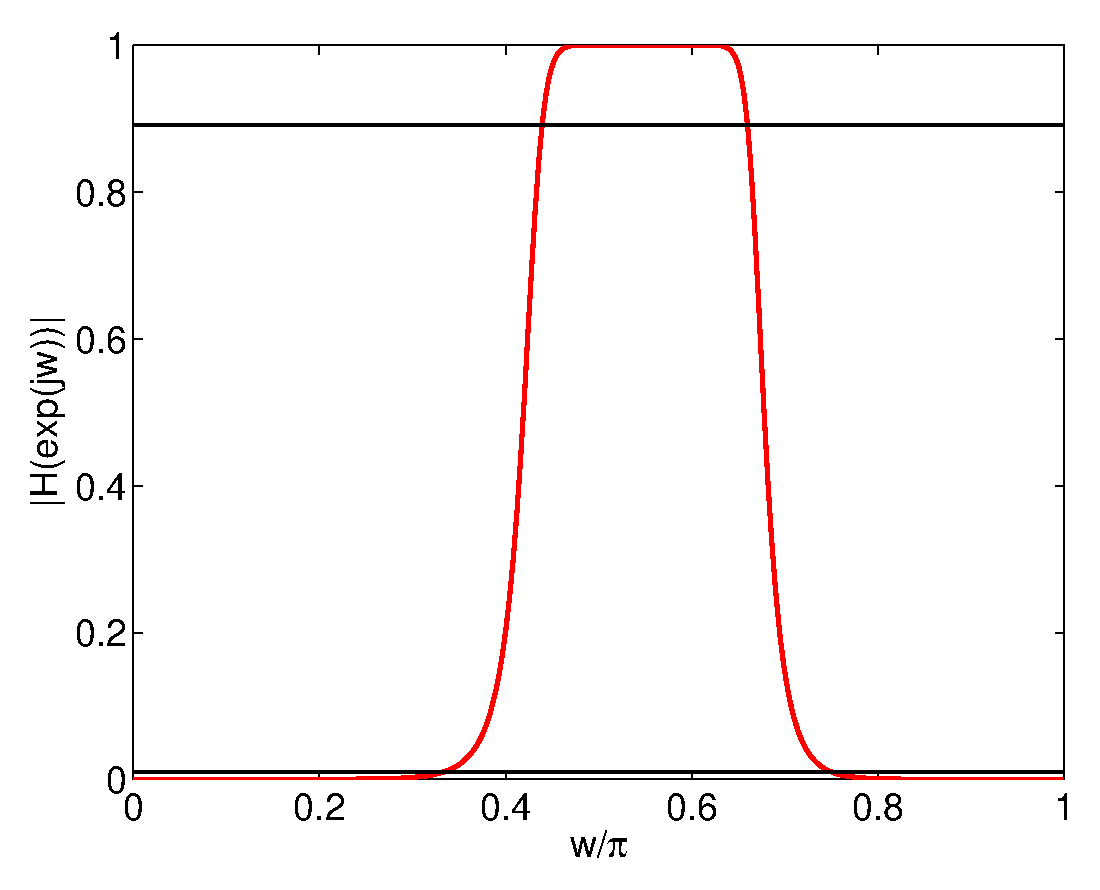
\includegraphics[width=3.8cm]{Figures/FiltroDiscretoPBanda_Butter.eps}
 \end{column}
 \end{columns}

\end{frame}

%%%%%%%%%%%%%%%%%%%%%%%%%%%%%%%%%%%%%%%%%%%%%%%%%%%%%

\begin{frame}
\frametitle{Relaciones espectrales discretas}

\begin{itemize}
\footnotesize
\item La transformación espectral discreta $z=F(\hat z)$ permite obtener a partir de un filtro discreto paso bajo $H_{LP}(z)$  otro filtro discreto$^1$ (paso alto, paso banda, supresor de banda) $H(\hat z)=H_{LP}(z)|_{z=F(\hat z)}$.
\begin{itemize}
\footnotesize

\item Filtro paso alta: $z^{-1}=-\frac{\hat z^{-1}+\lambda}{1+\lambda \hat z^{-1}}$, con
$\lambda=-\frac{cos((w_c-	\hat w_c)/2)}{cos((w_c+	\hat w_c)/2)}$



\item Filtro paso banda: $z^{-1}=-\frac{\hat z^{-2}-\frac{2\lambda \rho}{\rho+1}\hat z^{-1}+\frac{\rho-1}{\rho+1}}{\frac{\rho-1}{\rho+1}\hat z^{-2}-\frac{2\lambda \rho}{\rho+1}\hat z^{-1}+1}$,

$\lambda=\frac{cos((\hat w_{c2}+	\hat w_{c1})/2)}{cos((\hat w_{c2}-	\hat w_{c1})/2)}$, $\rho=\cot((\hat w_{c2}-\hat w_{c1})/2)\tan(w_c/2)$

\item Filtro supresor banda: $z^{-1}=\frac{\hat z^{-2}-\frac{2\lambda}{\rho+1}\hat z^{-1}+\frac{1-\rho}{\rho+1}}{\frac{1-\rho}{\rho+1}\hat z^{-2}-\frac{2\lambda}{\rho+1}\hat z^{-1}+1}$,

$\lambda=\frac{cos((\hat w_{c2}+\hat w_{c1})/2)}{cos((\hat w_{c2}-\hat w_{c1})/2)}$, $\rho=\tan((\hat w_{c2}-\hat w_{c2})/2)\tan(w_c/2)$


\end{itemize}

\item Con Matlab$^{2}$
\begin{itemize}
\footnotesize
\item \texttt{[npa,dpa]=iirlp2hp(numlp,denlp,wplp,wphp)}
\item \texttt{[npa,dpa]=iirlp2bp(numlp,denlp,wplp,[wp1d,wp2d])}
\item \texttt{[nbs,dbs]=iirlp2sp(numlp,denlp,wslp,[ws1d,ws2d])}
\end{itemize}
\end{itemize}

\vspace{-0.2cm}
\rule{10cm}{0.4pt}

\scriptsize
$^1$También existe una relación espectral que permite transformar un filtro paso bajo en otro paso bajo, que se utiliza para cambiar las especificaciones en frecuencia de un filtro paso baja ya diseñado.

$^2$ Las frecuencias tienen que estar  normalizadas entre $[0,1]$ que se corresponden a los valores discretos entre $[0,\pi]$


\end{frame}



\begin{frame}
\frametitle{Ejemplo de un filtro  IIR paso banda}
\footnotesize

\footnotesize
\color{olivegreen} Diseñar con el procedimiento 2 un IIR de Butterworth paso banda con las siguientes características: bordes normalizados de la banda de paso 0.45$\pi$ y 0.65$\pi$, bordes normalizados de la banda supresora 0.3$\pi$ y 0.75$\pi$, rizo paso banda 1dB, atenuación mínima banda supresora 40 dB.
\color{gray}
\vspace{0.1cm}

1)  Características del filtro continuo paso banda $H_a(s)$, usando $\hat w_{a}=tan(w_{d}/2)$  :

$\begin{array}{llll}\hat w_{p1a}=0.8541 &\hat w_{p2a}=1.6319  & \hat w_{s1a}=0.5095 & \hat w_{s2a}=2.4142
\end{array}$

\vspace{0.1cm}

2) Obtener las especificaciones del filtro continuo paso baja $H_{LP}(s)$:

\vspace{0.1cm}

\hspace{0.25cm}$\hat w_{s1a}=\frac{1.3938}{w_{s2a}}=0.5772$, $\hat w_0=1.1806$, $w_p=1$, $w_{s}=2.3617$


\vspace{0.1cm}

\begin{columns}[T]
 \hspace{0.2cm}\begin{column}{7.7cm}
3) Diseño filtro Butterworth

\vspace{0.1cm}

\hspace{0.25cm}\texttt{[N,wn]=buttord(1,2.3617,1,40,'s')}

\hspace{0.25cm}\texttt{[nlp,dlp]=butter(N,wn,'low','s')}

\vspace{0.1cm}

 4) Seguir el procedimiento 2:

 \vspace{0.1cm}

  \hspace{0.25cm}\texttt{[nlpz,dlpz]=bilinear(nlp,dlp,0.5);}

\visible<2->{
  \hspace{0.25cm}\texttt{[Hlpw,w]=freqz(nlpz,dlpz);}

  \hspace{0.25cm}\texttt{plot(w/pi,abs(Hw))}

   \hspace{0.25cm}\texttt{plot(w/pi,10\^ (-1/20)*ones(length(w),1))};

  }

 \visible<3->{
  \hspace{0.25cm}\texttt{a=ginput(1);} \hspace{0.25cm}\texttt{wp=a(1);}}

  \hspace{0.25cm}\texttt{wpasod=[0.45,0.65];}


 \hspace{0.25cm}\texttt{[nz,dz]=irrlp2bp(nlpz,dlpz,wp,wpasod)}


 \end{column}
 \hspace{-0.5cm}\begin{column}{3.8cm}
\only<2-3|handout=0>{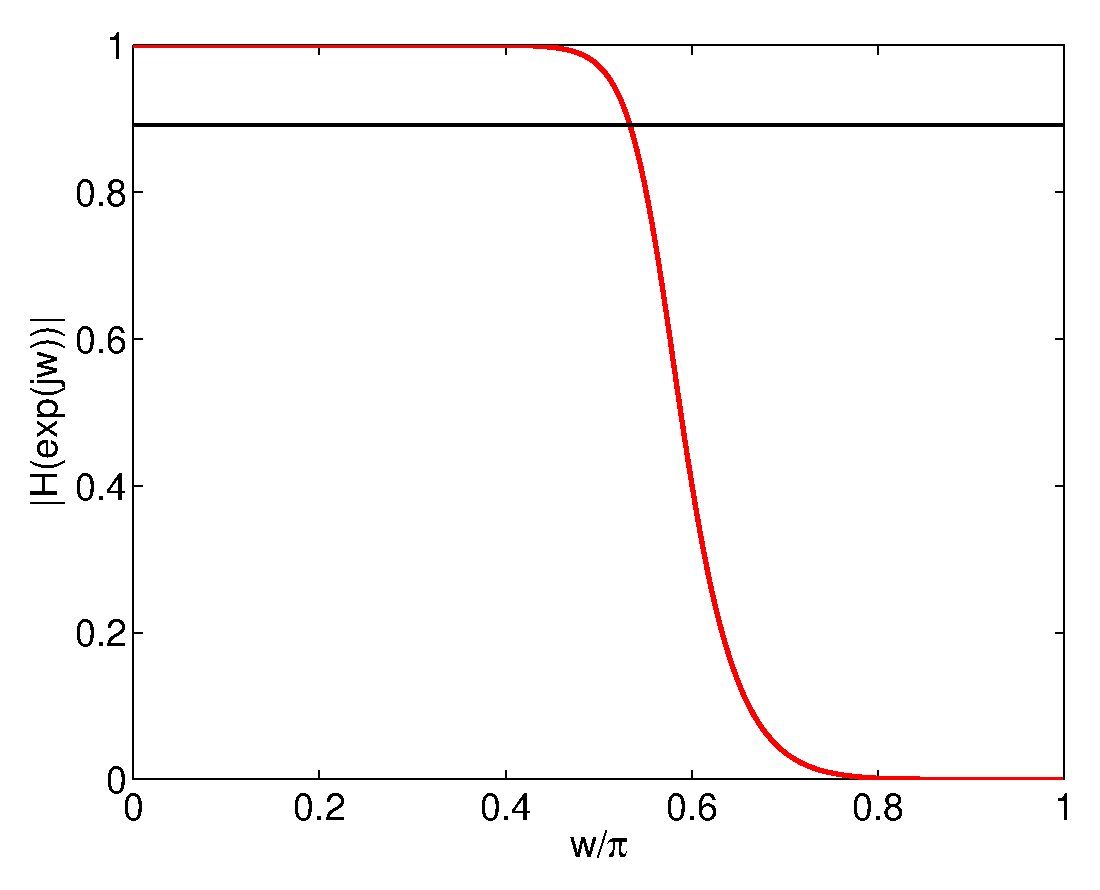
\includegraphics[width=3.8cm]{Figures/FiltroDiscretoPBanda_Butter21.eps}}
\visible<4->{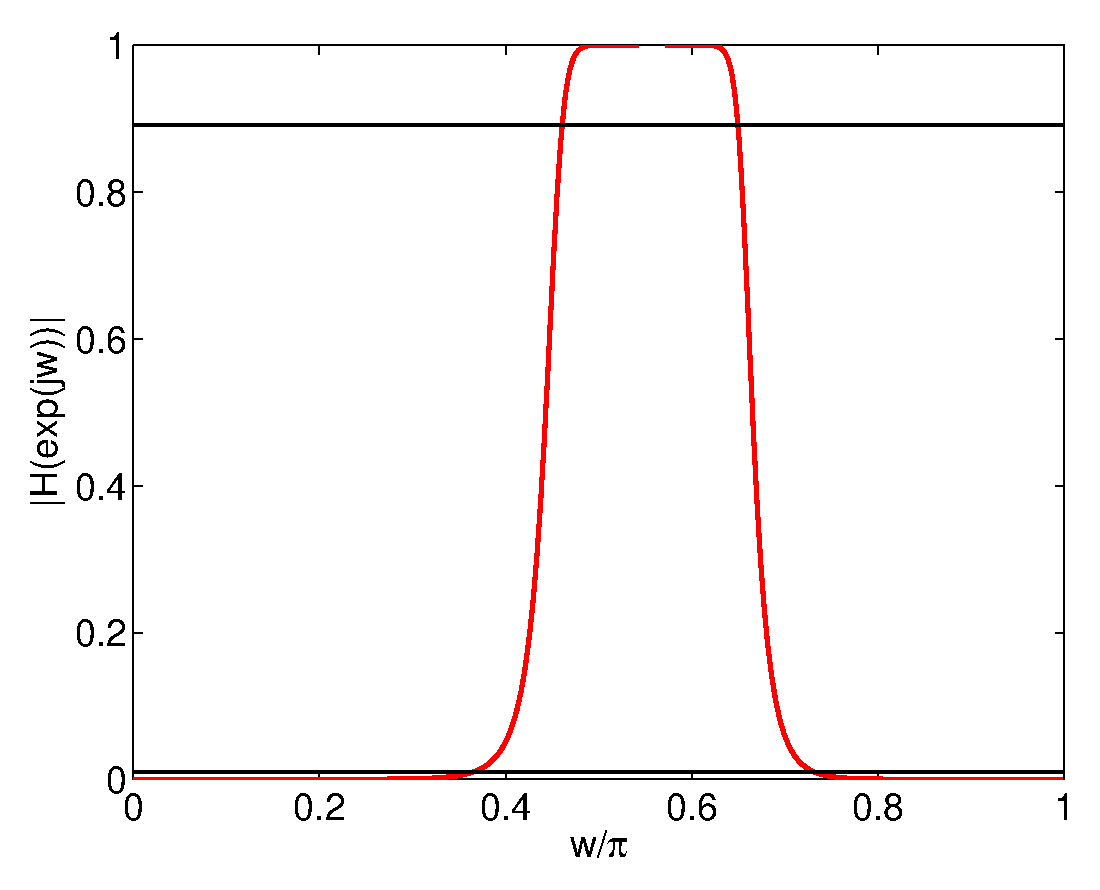
\includegraphics[width=3.8cm]{Figures/FiltroDiscretoPBanda_Butter22.eps}}

 \end{column}
 \end{columns}

\end{frame}

%%%%%%%%%%%%%%%%%%%%%%%%%%%%%%%%%%%%%%%%


\begin{frame}
\frametitle{Diseño de filtros  IIR con Matlab}
\footnotesize
\begin{itemize}
\item Matlab permite realizar directamente el diseño de los filtros discretos, sin necesidad de realizar los pasos intermedios.
\item Para ello, hay que poner en las funciones que ya conocemos las frecuencias normalizadas [0,1] y eliminar la llamada a 's'.

\item Veamos un ejemplo con las funciones de Chebyshev de tipo II
\begin{itemize}
\item \alert{\texttt{[N,wn]=cheb2ord(wp,ws,alphap,alphas);}}

\vspace{0.1cm}

{\footnotesize
\hspace{0.5cm}Paso bajo: wp=0.3, ws=0.5;

\vspace{0.1cm}

\hspace{0.5cm}Paso alto: wp=0.5, ws=0.3;

\vspace{0.1cm}

\hspace{0.5cm}Paso banda: wp=[0.5 0.7], ws=[0.4 0.8];

\vspace{0.1cm}

\hspace{0.5cm}Eliminación de banda: wp=[0.5 0.7], ws=[0.55 0.65];}

\vspace{0.1cm}

\item\alert{\texttt{[num,den]=cheby2(N,alphas,wn,tipo);}}

\vspace{0.1cm}

\hspace{0.5cm}tipo: 'low', 'high', nada, 'stop'

\end{itemize}


\item Los resultados de Matlab coinciden con los obtenidos a través del procedimiento 1.

\end{itemize}

\end{frame}





\begin{frame}
\frametitle{Ejemplo de un filtro  IIR paso banda}
\footnotesize

\footnotesize
\color{olivegreen} Diseñar directamente con Matlab un IIR de Butterworth paso banda con las siguientes características: bordes normalizados de la banda de paso 0.45$\pi$ y 0.65$\pi$, bordes normalizados de la banda supresora 0.3$\pi$ y 0.75$\pi$, rizo paso banda 1dB, atenuación mínima banda supresora 40 dB.
\color{gray}
\vspace{0.1cm}


\vspace{0.1cm}

\begin{columns}[T]
\begin{column}{6cm}
\lstinputlisting{./Matlab/ButterDCode.m}


 \end{column}
\hspace{-0.5cm} \begin{column}{4.5cm}
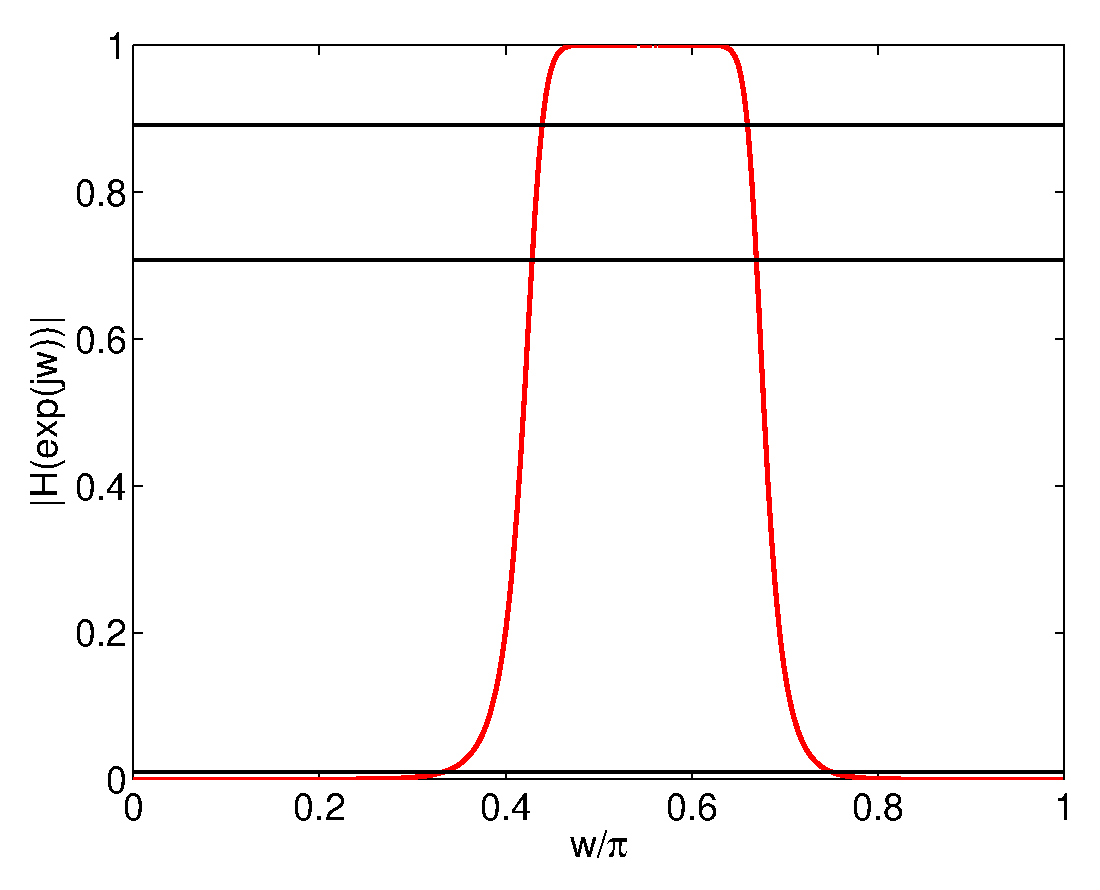
\includegraphics[width=4.5cm]{Figures/FiltroDiscretoPBanda_ButterMatlab.eps}

 \end{column}
 \end{columns}

\end{frame}
